\chapter{Circuits` performance improvement by reducing internal power loss}\label{front}
%\addcontentsline{toc}{chapter}{Apendix}	% to be visible in TOC but unnuvered

\indent In this Chapter it is shown that power loss reduction allows to extend the functional range of a circuit on an example of a low-cost impedance tuner for push-pull transistor measurement. The usable range of realizable impedances is increased by replacing the core circuit from a larger and more lossy rat-race coupler to a six times smaller coupled-line coupler  to allow for measurement of power transistors featuring very low input/output impedance, which in addition requires shorter lengths of the tuning sliding loads. Such measurements are in many cases crucial for the design of high-power microwave amplifiers as in the developed high-power transceiver front-end where the proposed tuner was used to find  terminating impedances at the transistor`s input and output for the maximum power. The results of the conducted research have been a subject of a conference paper presented at \textit{Radio and Wireless Symposium RWS`16} under the auspices of \textit{Institute of Electrical and Electronics Engineers} and a technical report on the realization of \textit{RF Pulsed Power Amplifier} work package within \textit{Air traffic control system of the new generation ADS-B/MLAT} project granted by the National Centre for Research and Developement under the POIR program to Avionix Engineering Sp. z o. o., ID project number POIR.01.01.01-00-0169/15, which constitute the Chapter.
\\
\indent A low-cost impedance tuner is shown in Section \ref{rws_tuner} being well suitable for load-/source-pull transistor measurements. The proposed circuit consists of a 3-dB quadrature coupled-line directional coupler with tuning components realized as shorted microstrip line sections with appropriate sliding shorting elements, which allow to provide any desired impedance. The theoretical analysis of the proposed circuit has been performed and the principle of circuit’s behavior has been explained. An exemplary impedance tuner has been designed, manufactured and measured. The obtained measurement results showed the Voltage Standing Wave Ratio (VSWR) as high as 41:1 translating to a load impedance as low as $Z_{L}$ = 1.26 $\Omega $ proving usefulness and demonstrating the advantages of the presented approach.
\\
\indent Following, a custom power amplifier for the product components “Automatic dependent surveillance – broadcast (ADS-B) vehicle transponder” and “MODE-S interrogator” was of need. An RF power amplifier working in pulsed mode with minimum of 20 W peak output power for efficient Pulse-Position Modulation (PPM) amplification is designed and described in Section \ref{avionix_report} to be used as a part of the ADS-B vehicle transponder where small size and low power consumption are of importance. Moreover, the amplifier is integrated into a transceiver front-end module with a RX/TX switch for the operation with a single antenna. The developed module consist of an MMIC pre-amplifier module and an RF transistor based power amplifier. The utilized transistor was measured during the design process using source and load-pull technique with low-cost impedance tuners to allow for the determination of input and output terminating impedances that ensure maximum power amplification. Measurement results show compliance of the manufactured front-end with the design requirements.
% RF transisor NXP MRFE6VS25 on a short mount, VD = 40V, VG = 2.5V, Pin = 0 dBm + wzmacniacz + 30 dBm
%  1030 MHz bramka - stroik Z=2.52-j6.75 Ohm, Z=|0.905| -164.55deg
%  1030 MHz dren - stroik Z=5.98-j1.07 Ohm, Z=|0.786| -177.5deg
%  1090 MHz bramka - stroik Z=9.4-j3.9 Ohm, Z=|0.685| -170.7deg
%  1090 MHz dren - stroik Z=4.93-j2.78 Ohm, Z=|0.82| -177.3deg

\cleardoublepage

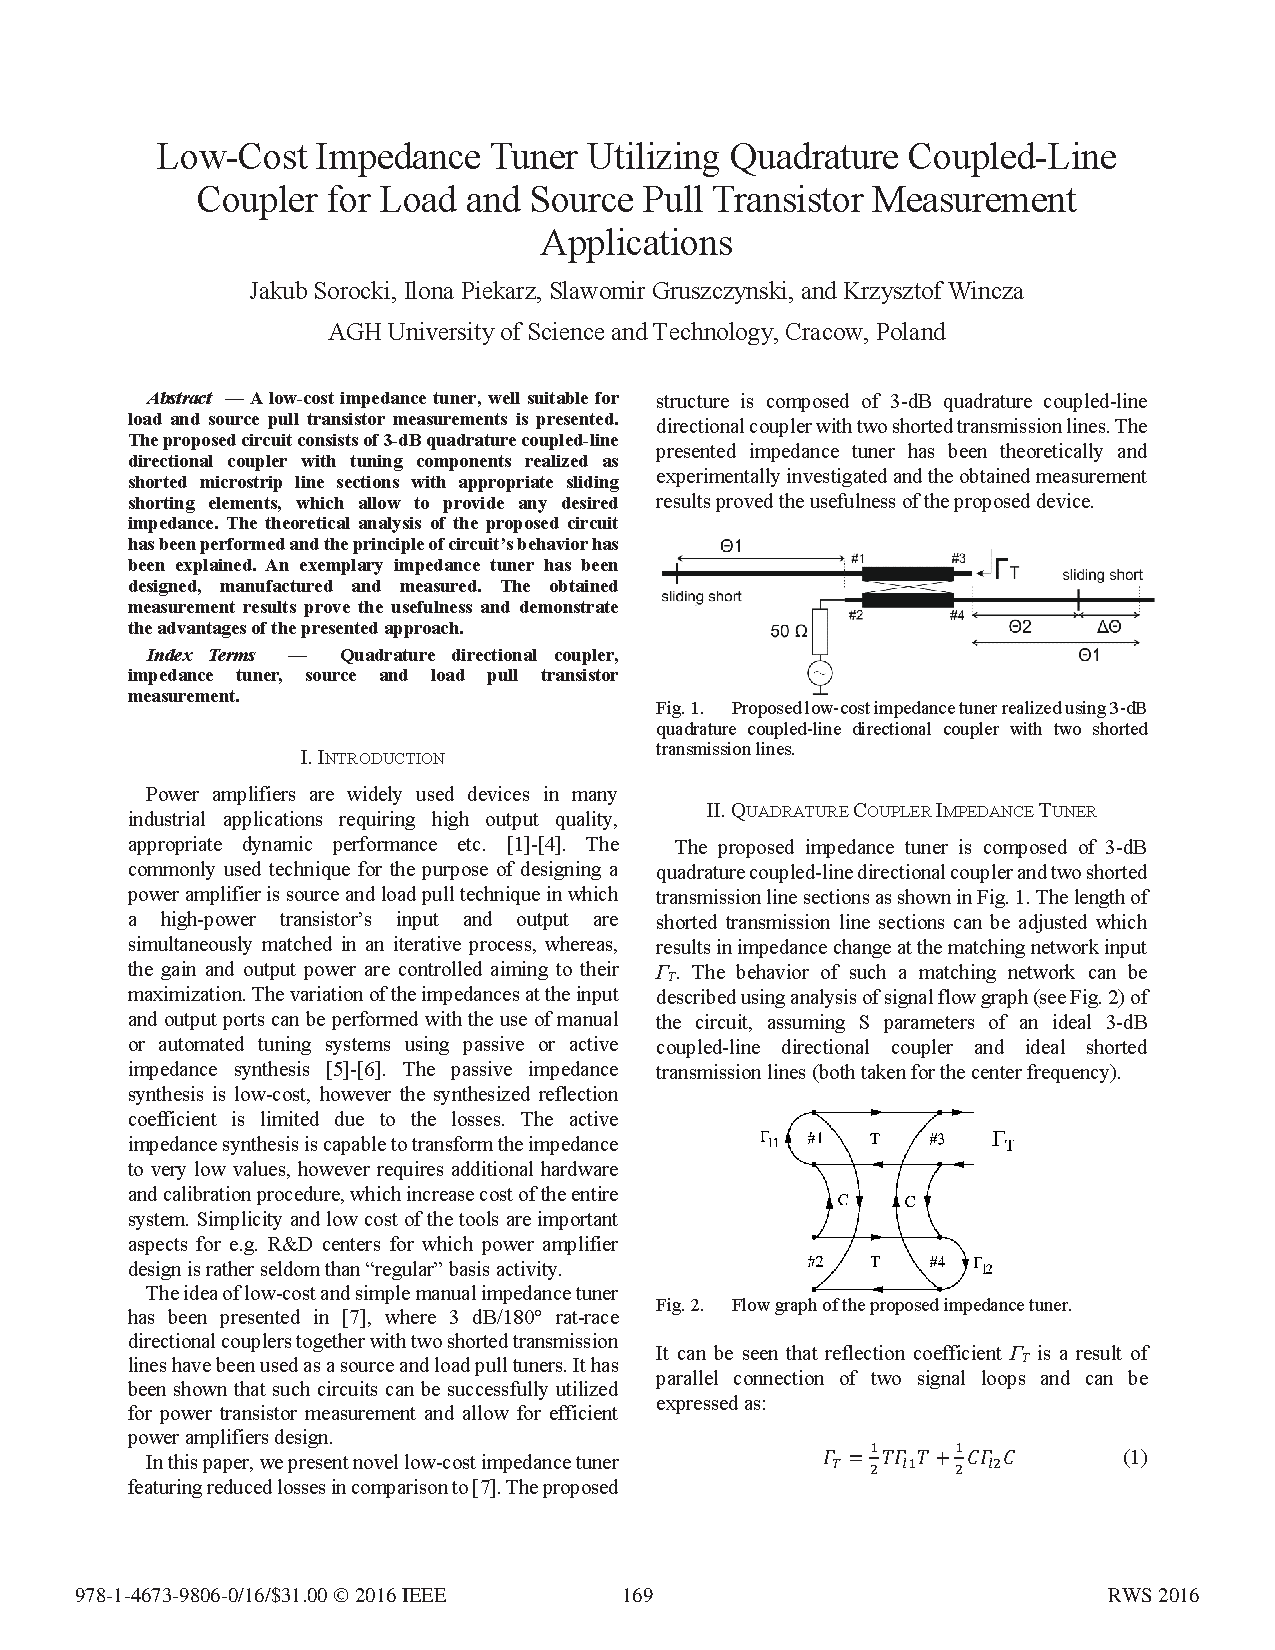
\includepdf[pages=-,addtotoc={1,section,1,Low-cost impedance tuner utilizing quadrature coupled-line coupler for load and source pull transistor measurement applications,rws_tuner}, pagecommand={}, scale=.97]{chapter_6/rws_tuner.pdf}

\cleardoublepage

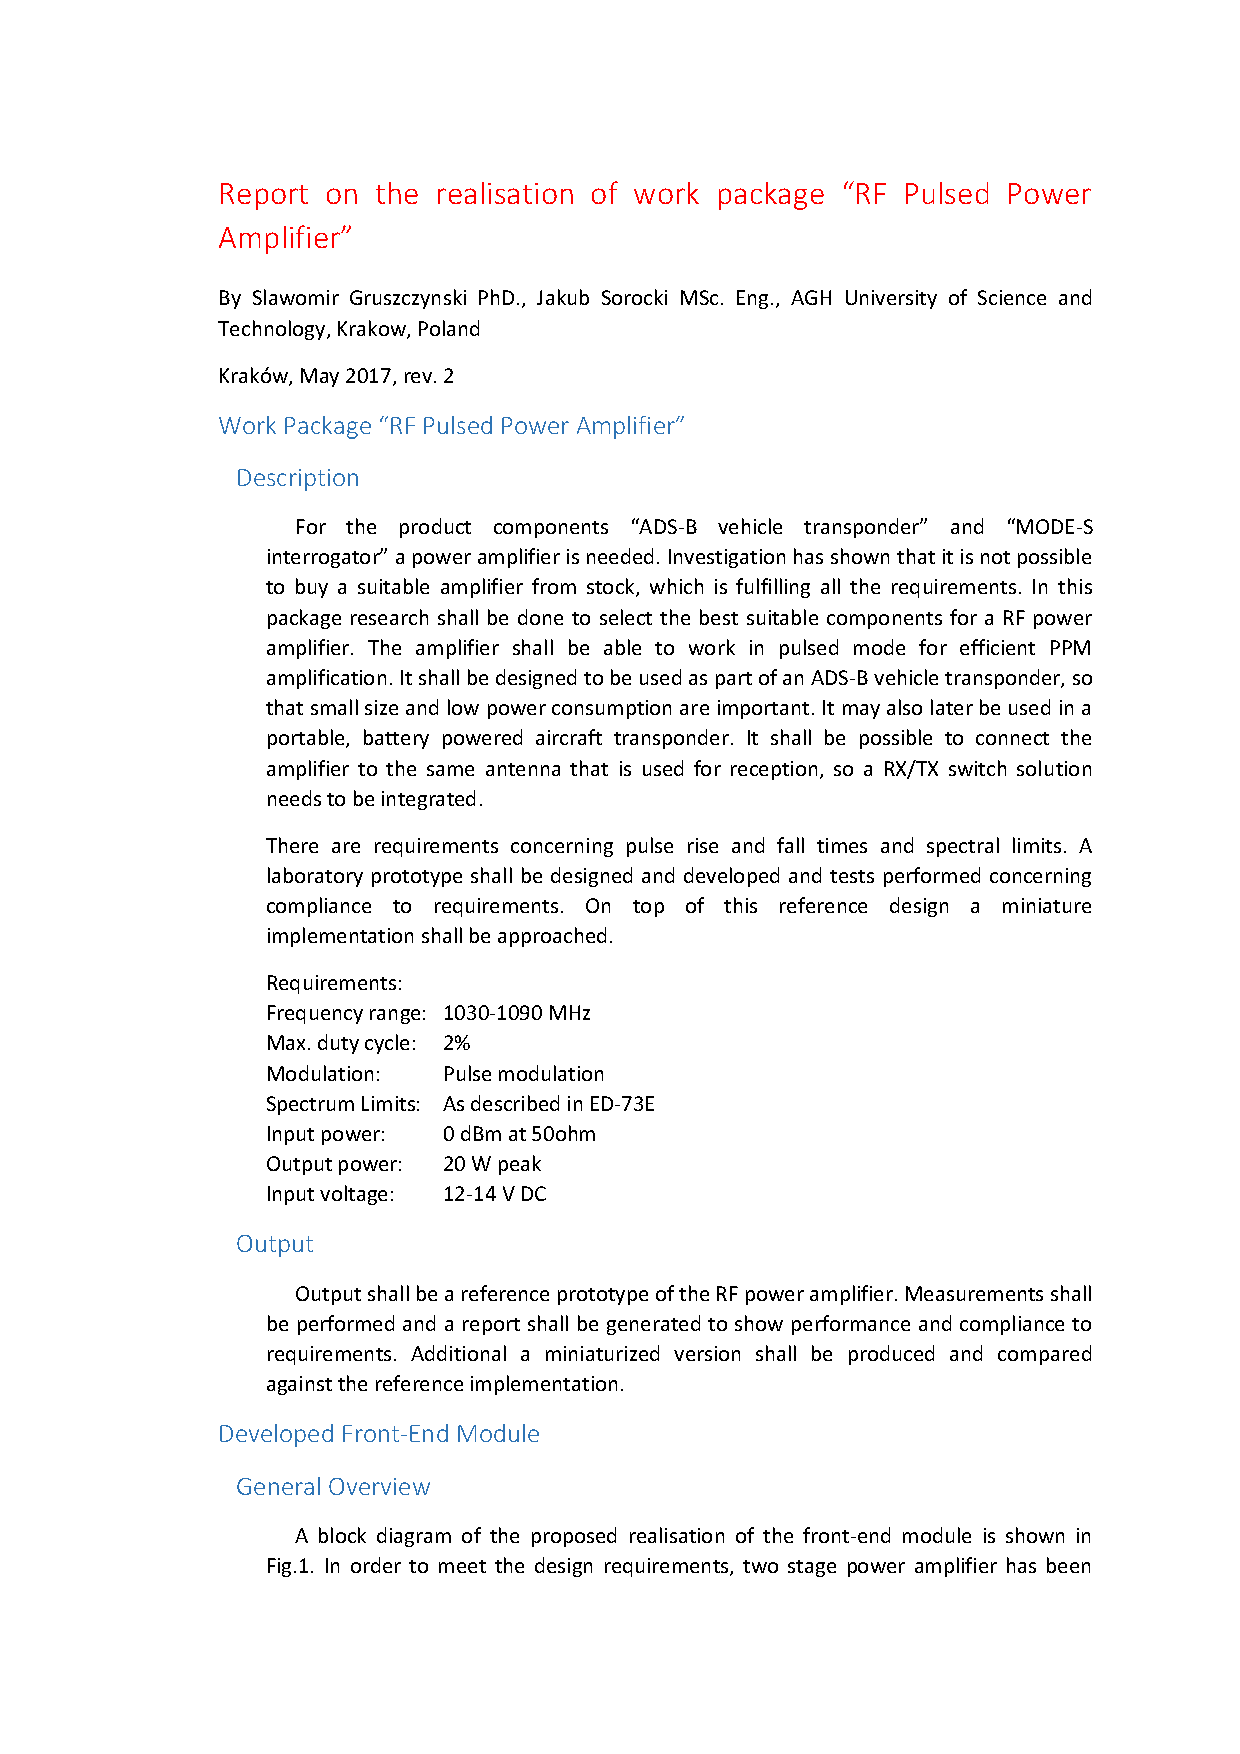
\includepdf[pages=-,addtotoc={1,section,1,Report on the realization of work package \textit{RF Pulsed Power
Amplifier} within the \textit{Air traffic control system of the new generation ADS-B/MLAT} project,avionix_report}, pagecommand={}, scale=.97]{chapter_6/avionix_report.pdf}

\cleardoublepage